\documentclass{beamer}

\usepackage[ngerman]{babel}
\usepackage{graphicx}
\usepackage{hyperref}


% Example here:
% https://github.com/josephwright/beamer/blob/main/doc/solutions/conference-talks/conference-ornate-20min.de.tex

\mode<presentation>
{
    \usetheme{Singapore}
%\usetheme{AnnArbor}
%\usecolortheme{beaver}
}

\title{Kolloquium Pflichtenheft}
\subtitle{SEP WS 2021/2022}

%\titlegraphic{
\includegraphics[width=5cm]{../../docs/Pflichtenheft/graphics/LasEs-logo}}

\date{\small 30. November 2021}
\logo{
\includegraphics[width=1.5cm]{../../docs/Pflichtenheft/graphics/LasEs-logo}}

\author{\textbf{Team 2} \\ \small {Johann Schicho, Stefanie Gürster, Thomas Kirz,\\ Johannes Garstenauer, Sebastian Vogt} \\ \vspace{0.5cm}\emph{Phasenleiter: Johannes Garstenauer}\normalsize}


\begin{document}

    \begin{frame}
        \titlepage
    \end{frame}

    \begin{frame}{Gliederung}
        \tableofcontents
    \end{frame}


    \section{Änderungen zum Pflichtenheft und Entwurf}

    \begin{frame}{Änderungen}
        Vereinfachungen \& Übersichtlickeit
        (Um das Produkt für Sie besser zu gestalten haben wir einige Verbesserungen vorgenommen:)
        \begin{itemize}
            \item Neue Pakete zur Übersichtlichkeit und Einhaltung der selbstdefinierten Paketfunktionen
            z.B. persistence.internals zum Zugriff auf Konfig \& Res.Bundles, da repositories für entitäten gedacht sind.
            \item Verwendung des Standardlogger
            \item Facelets wurden zusammengelegt (z.B. Ansicht und Bearbeitung einer Einreichung)
            \item Pagination DTOs wurden simplifiziert
        \end{itemize}
        Verinfachungen machen die Implementation weniger zeitaufwendig.
        Übersichtlichkeit macht die Planung leíchter.
        Somit ist das Produkt günstiger für Sie.
    \end{frame}

    \begin{frame}{Ordnerstruktur}
        Übersichtlichkeit und Zugriffskontrolle
        \centering
        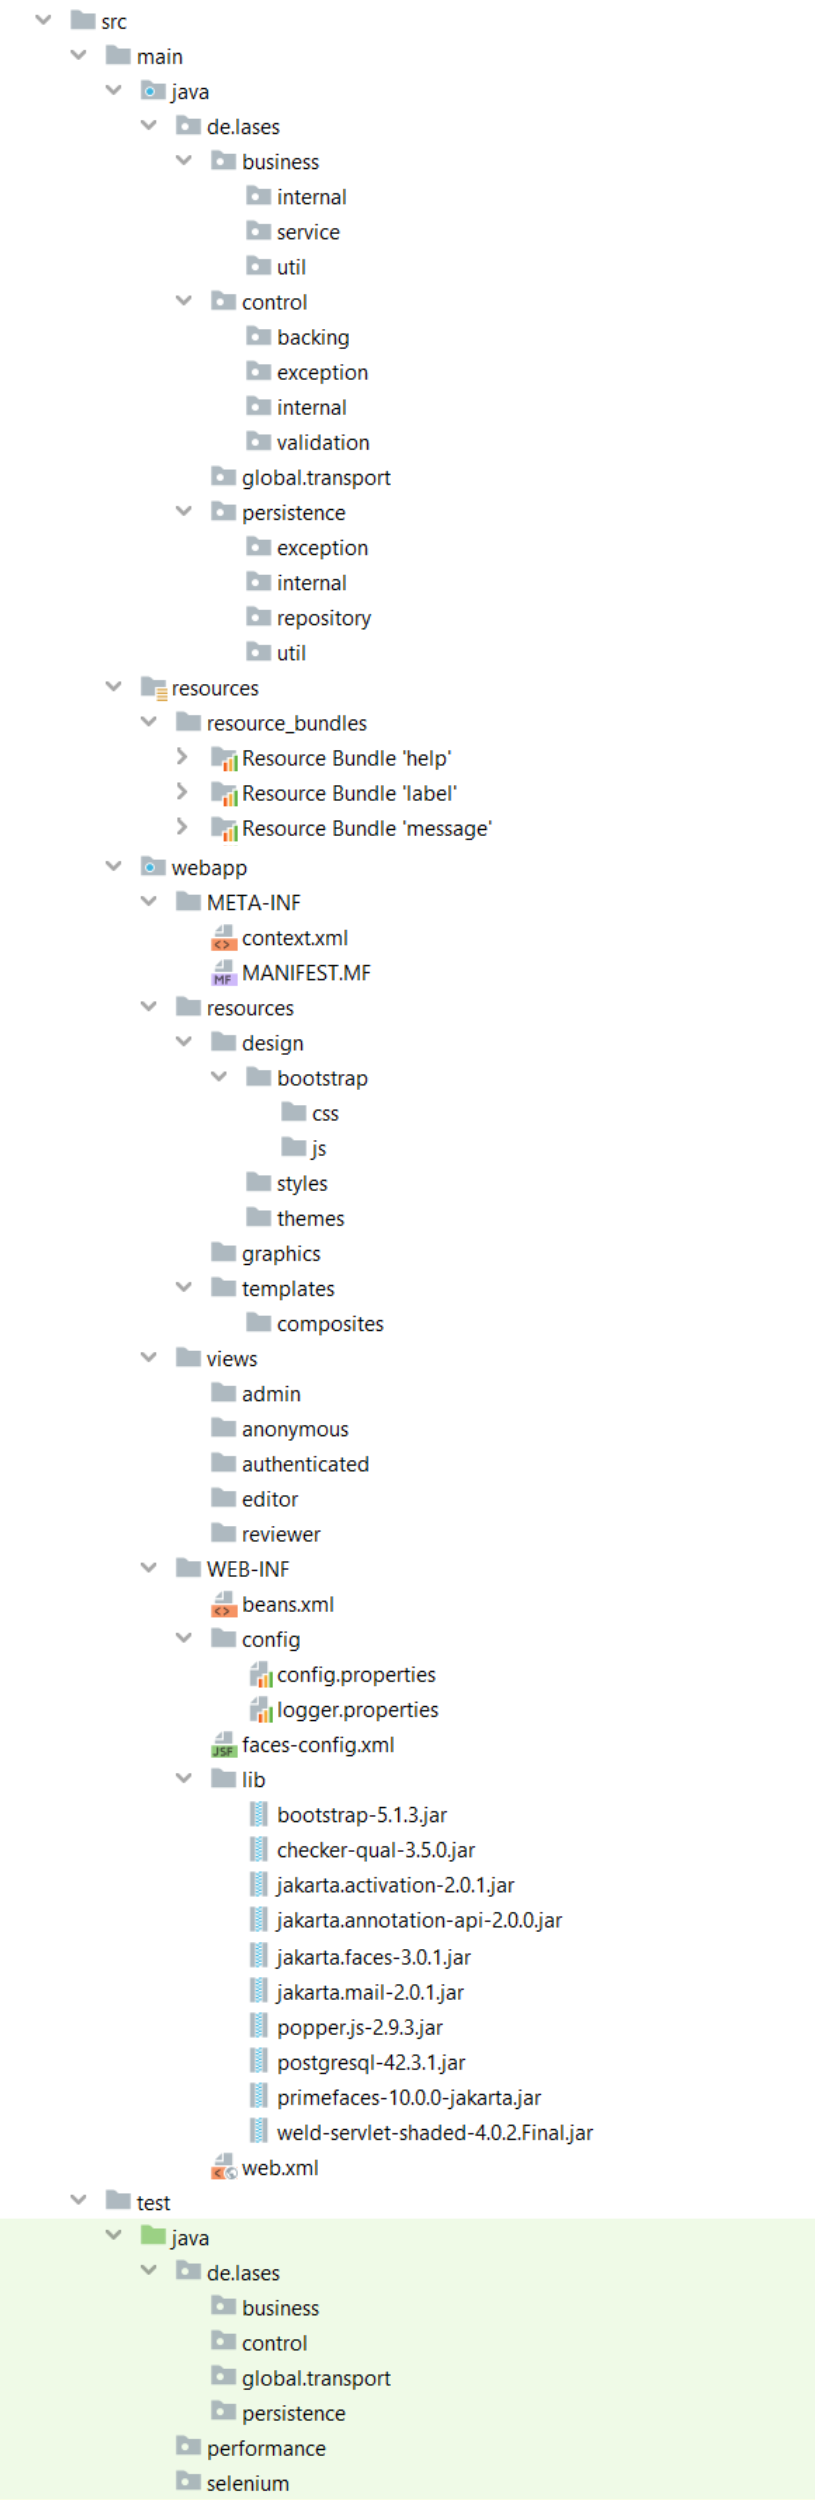
\includegraphics[height=1.1\textheight]{graphics/w2_folder_final}
        Ausschnitt ab ressources
        \begin{itemize}
            \item Labels, Tooltips und UI-Nachrichten in mehreren jew. einsprachigen Resource-Bundles.
            -> bietet Internationalisierbarkeit und leichtes Hinzufügen neuer Sprachen.
            \pause
            \item Konfigurationsdateien im \emph{WEB-INF}-Verzeichnis um sie vor unautorisierten
            Zugriffen schützen.
            \pause
            \item Tests nach Paketen, Performance und Selenium unterteilt, (Feine Unterteilung der Testpakete)
            um zu modularem Testing anzuregen.
        \end{itemize}
        \pause
        \centering
        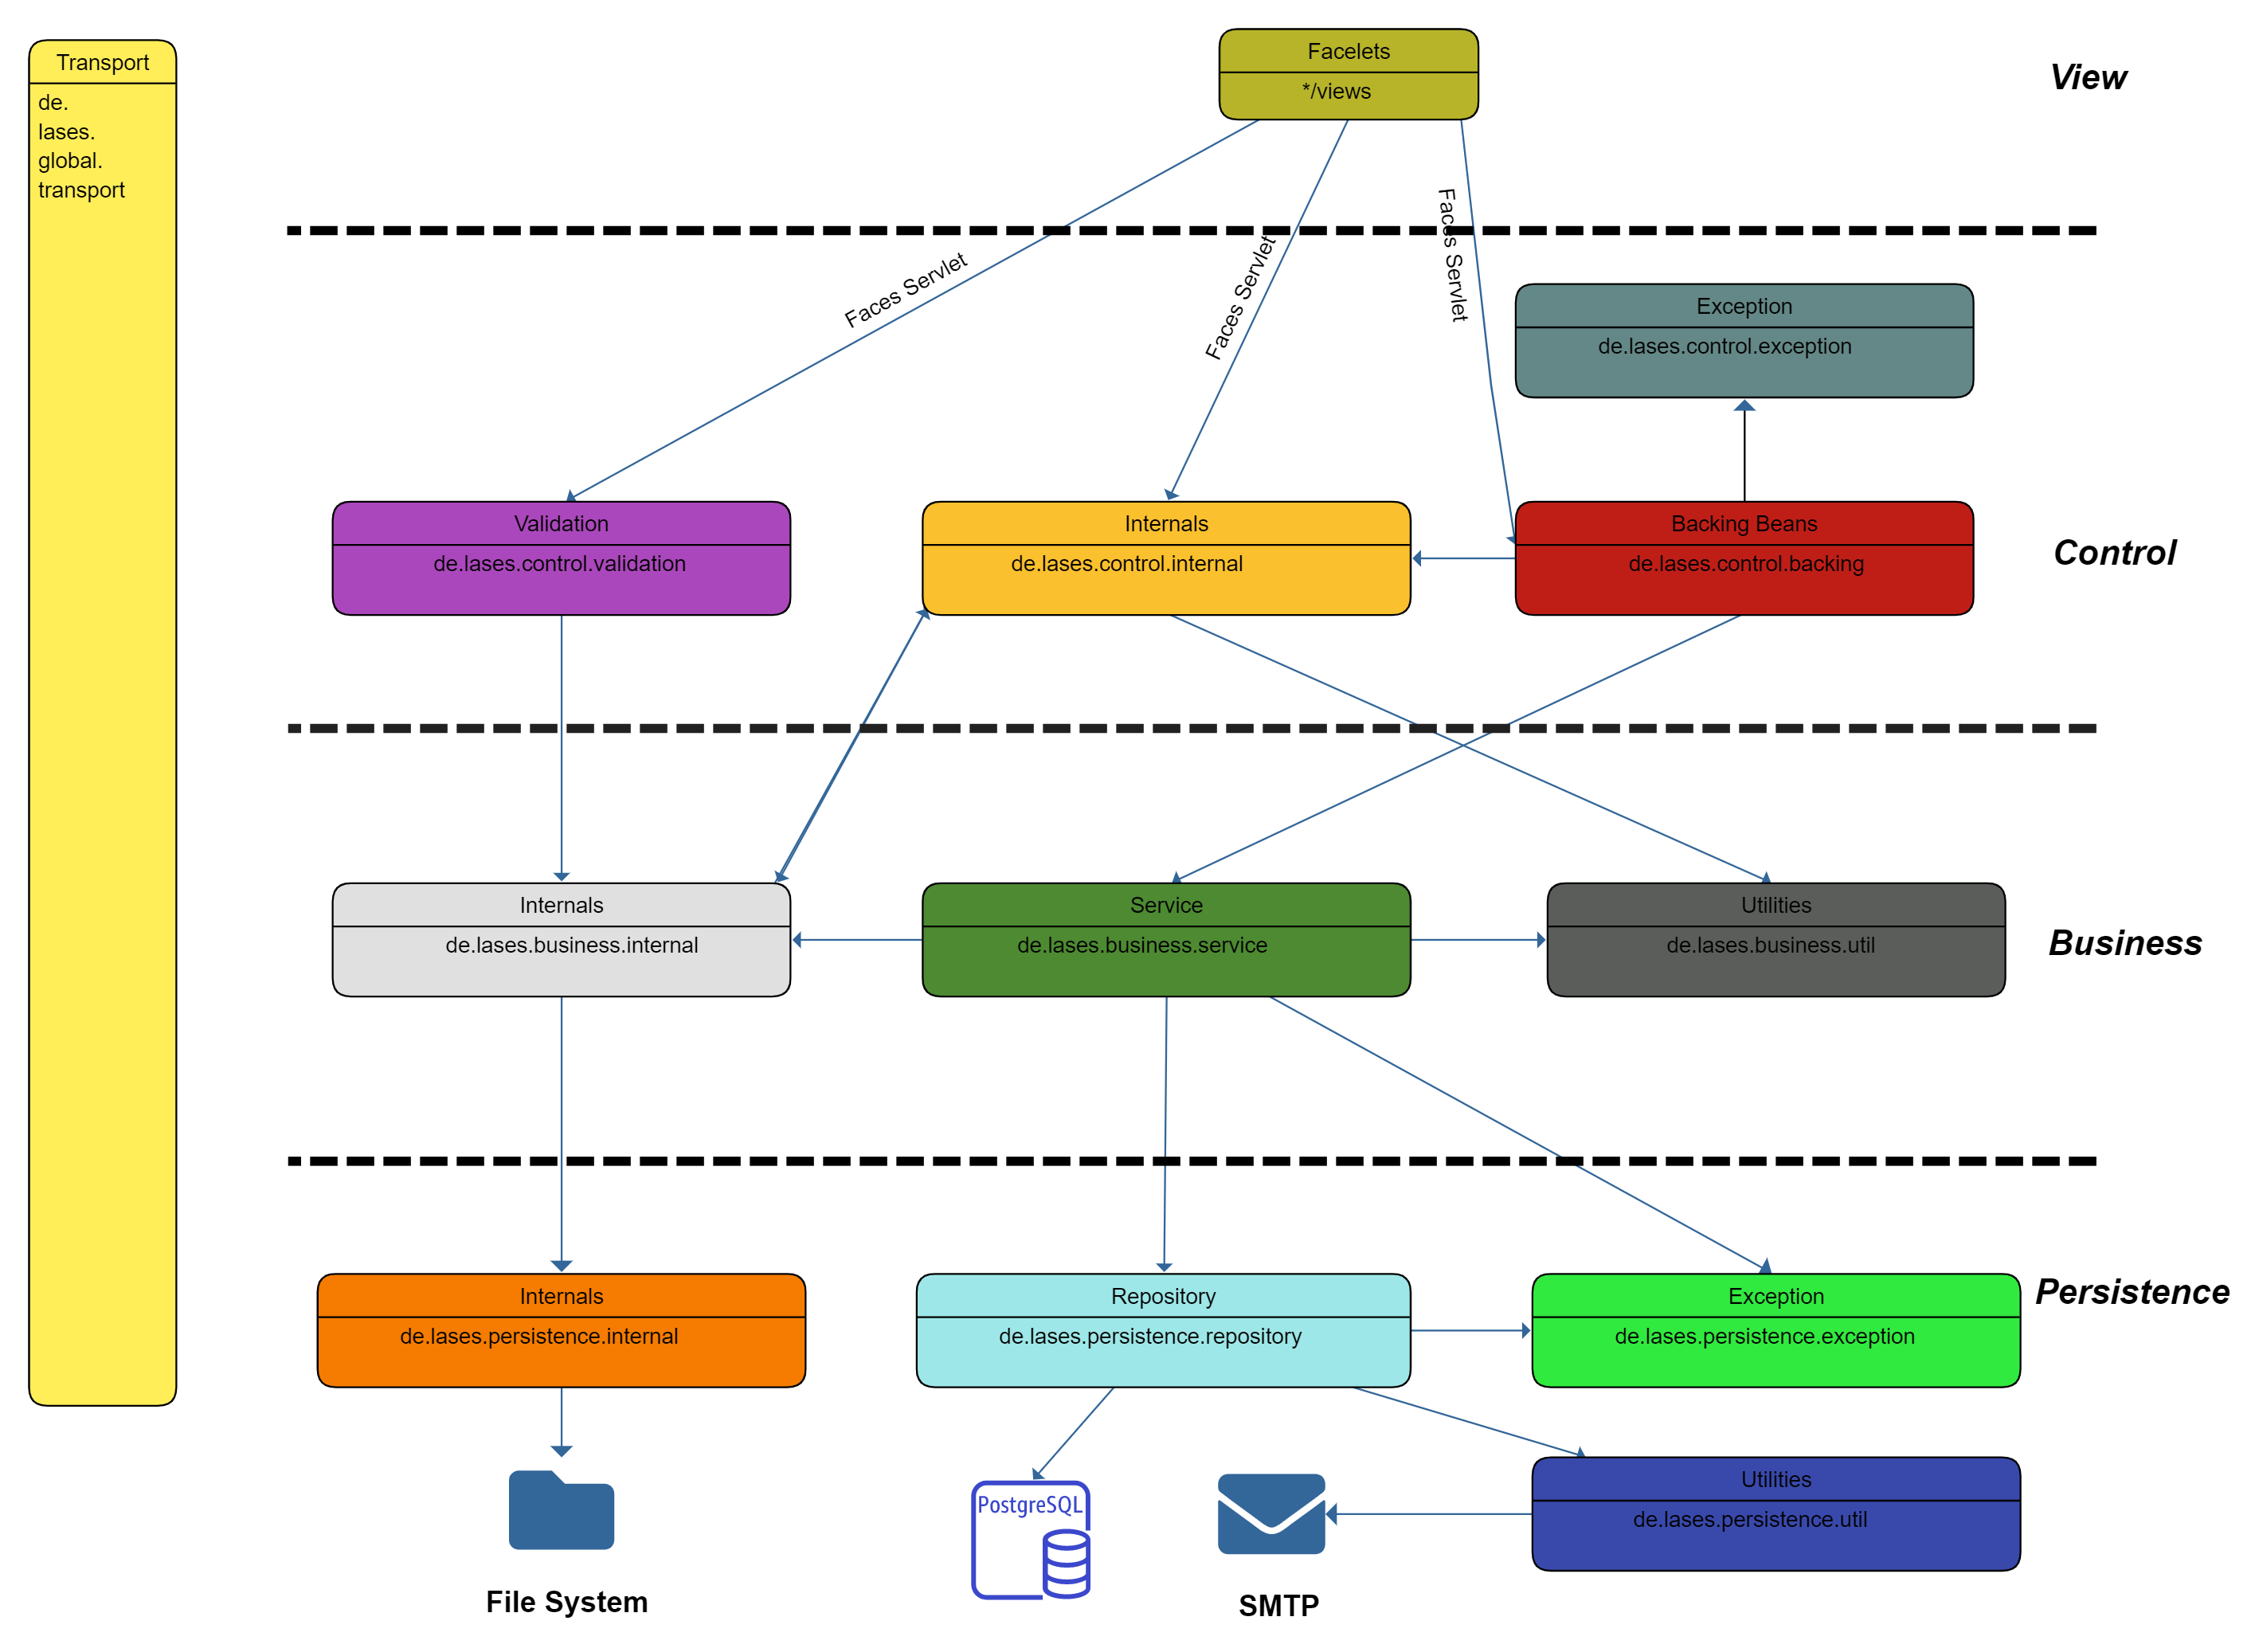
\includegraphics[height=1.1\textheight]{graphics/Paketdiagramm (15)}
        \begin{itemize}
            \item Größtenteils gleichgeblieben. Änderungen aus Punkt 1 wurden übernommen.
            \item Wir haben besonders darauf geachtet:
            \item Klare Trennung der Schichten, verständliche Interfaces und v.a. schwache Kopplung!
            \item Wir garantieren: Sie können diese Anwendung noch sehr lange verwenden,
            alle schichtenspezifischen Technolgien wie z.B. die PostGres-Datenbank
            oder Facelets von JSF sind komplett und problemlos austauschbar:
            \item Schichten wissen nichts voneinander ausser durch die Interfaces!
        \end{itemize}
    \end{frame}


    \section{Facelet}
    \begin{frame}{Lastenheft}
        \centering
        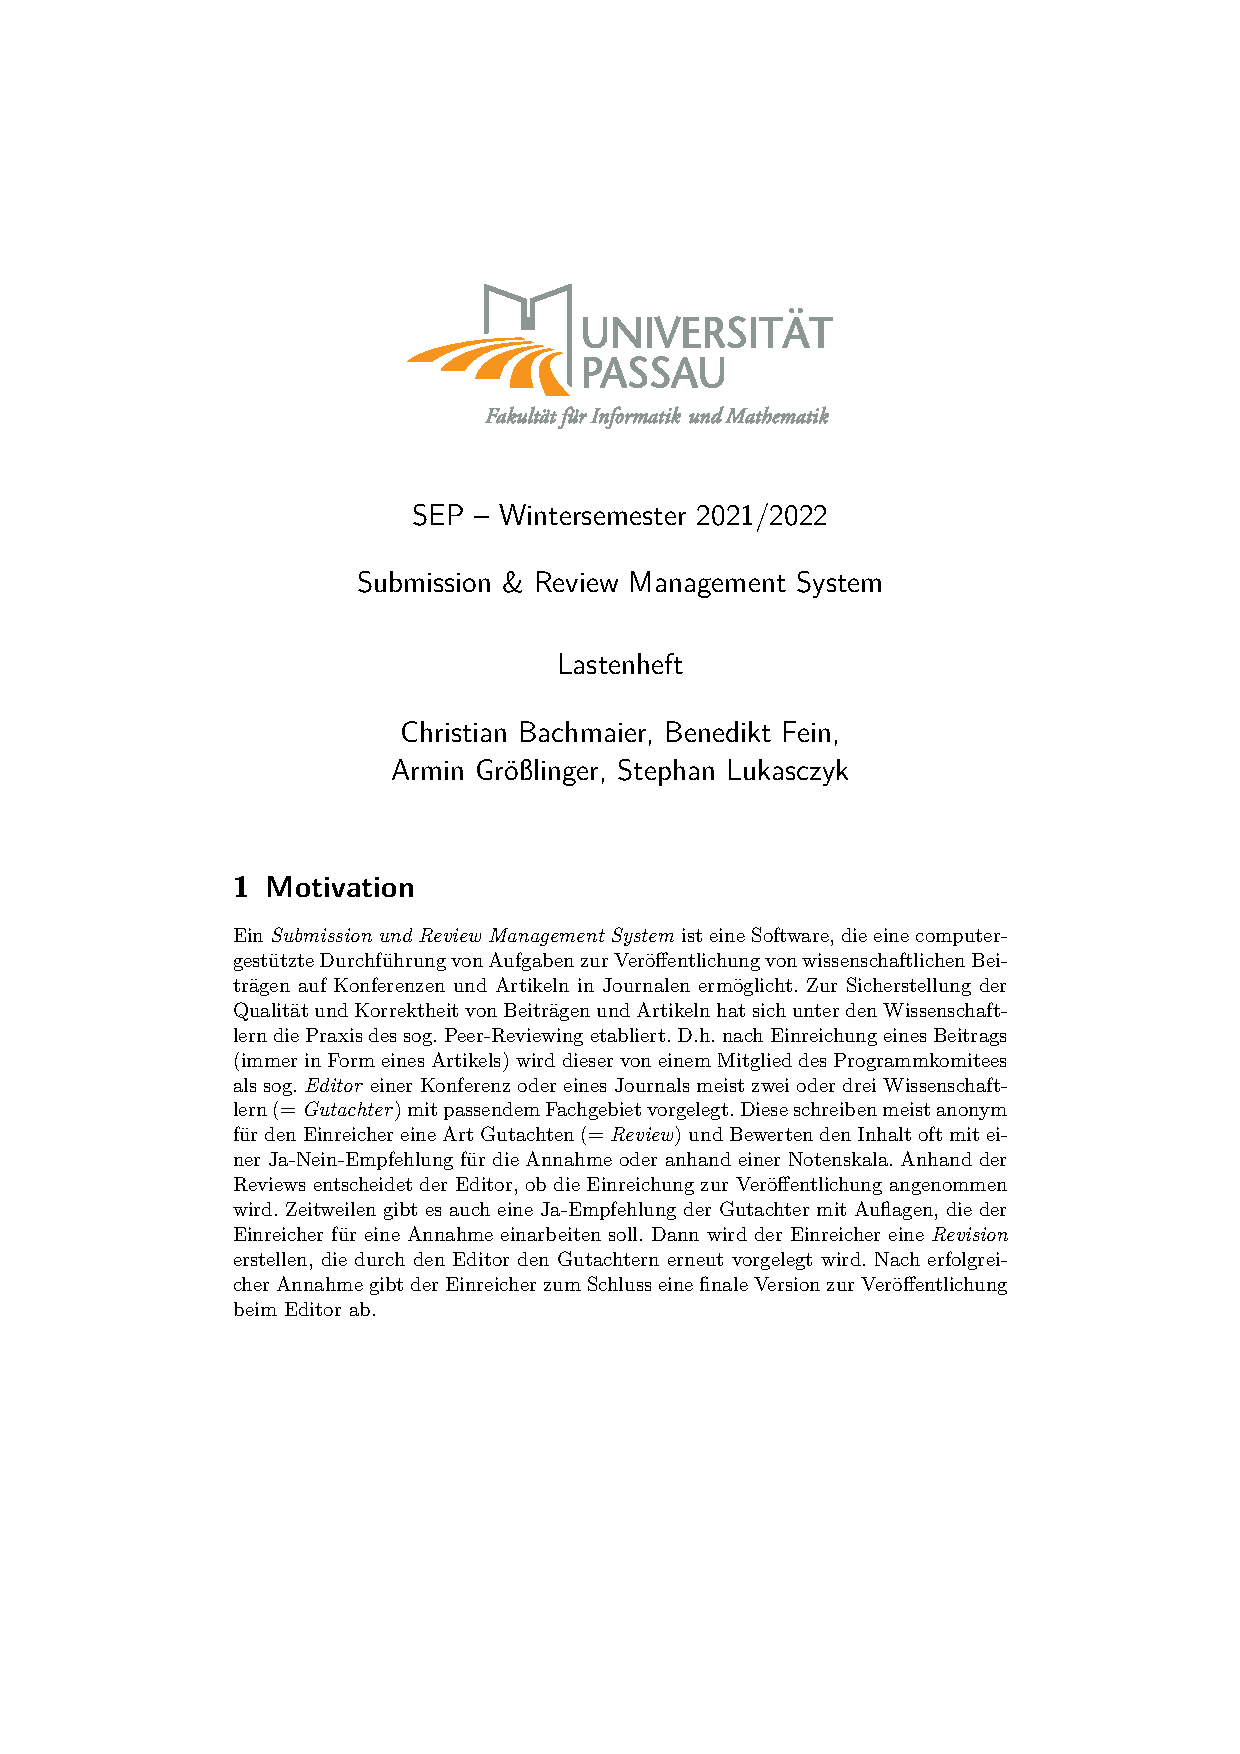
\includegraphics[height=1.1\textheight]{../../docs/Lastenheft/lastenheft}
    \end{frame}

    \subsection{Datenfluss}
    \begin{frame}{Lücken und Unklarheiten}

        Typische Klasse \textbf{Persistenzschicht} : \emph{SubmissionRepository}.
        \pause
        \begin{itemize}
            \item Keine Attribute
            \item Nur statische Methoden
            \item (Fast) jede Entität besitzt ein Repository.
            Fast zur Vereinfachung des Entwurfs.
            \item Bietet add(Submission, Transaction), change(Submission, Transaction)
            -> inheitliche und übersichtliche Interfaces:
            und get(Submission, Transaction) an.
            Obwohl Methodensignatur selbe Parameter: verschiedene Funktionsweise.
            Add: alle req. fields ohne id
            change: id + req. fields
            get: nur id
            -> Datenfluss ohne flache Parameter, gekapselt in DTOs
            -> Dieses DTO muss jeweils nur die Daten enthalten, welche zum Zeitpunkt des Aufrufs
            zur Verfügung stehen und die Daten welche zur Verarbeitung benötigt werden.
            \item Um das im Interface widerzuspiegeln gibt die JavaDoc das jeweils genau vor.
            \item Hier RaceConditions?
        \end{itemize}

        Typische Klasse \textbf{Businessschiht} : \emph{SubmissionService}.
        \pause
        \begin{itemize}
            \item informiert den Nutzer über Fehlerhaften Zustand aus unteren Schichten und in der Geschäftslogik
            über Events welche in der oberen Schicht zu FacesMessages  umgewandelt werden
            \item Bietet ebenfalls add(Submission), change(Submission)
            und get(Submission) an.
            \item Hohe Überdeckung zu Persistenzschicht, einheitliche und übersichtiliche Interfaces:
            \item Leichtere Implementation und Zurechtfinden.
            \item verwendet Transaktionen:
            \item um ACID Eigenschaften sicherzustellen: Atomarität, Konsistenz, Isolation, Dauerhaftigkeit
            ?und Race-Conditions zu vermeiden?
            \item @Dependent-Scoped
        \end{itemize}
    \end{frame}

    \subsection{Gespeicherte Sessioninformationen}
    \begin{frame}{Attribute}
        \begin{itemize}
            \item User-DTO mit ID
            -Immer nur mit ID? Wieso nur Id? (Auf mehr Daten kann man sich nicht verlassen, dass diese vorhanden sind: Minimum)
            -Welche Elemente gerendert werden ist immer davon Abhängig wer eine bestimmte Seite sieht.
            -Sicherheit: Hat diese Session Zugriff auf best. Seite?
            - Wieso nicht mehr in Session (Privilege z.B.)
            \pause
            \item Locale zur Internationalisierbarkeit.
            - Ist Locale abfragbar? Sparen wir uns hiermit Anfragen an den Browser?
        \end{itemize}
    \end{frame}


    \section{Konfiguration}
    \begin{frame}{Allgemeine Konfiguration}
        Hier ein kurzer Blick auf die allgemeine Konfiguration
        -Validatorenkonfiguration (Filesizes)
        -Pagination
        -Debug
        -Mail
        -DB
        \centering
        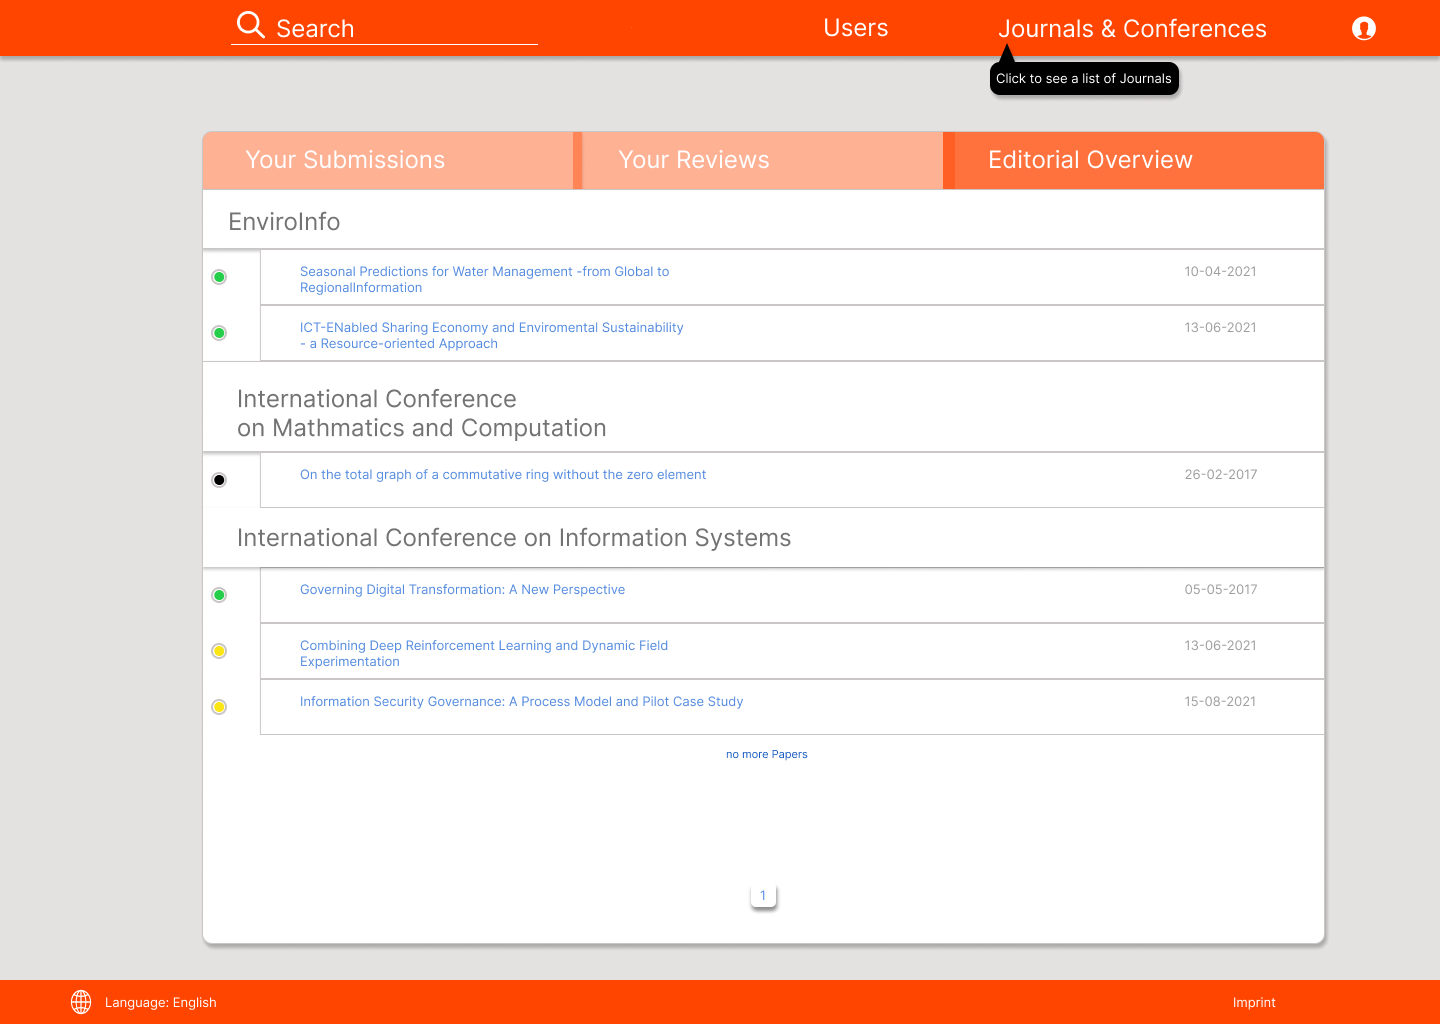
\includegraphics[height=0.75\textheight]{../../docs/Pflichtenheft/graphics/Homepage-png}
    \end{frame}

    \begin{frame}{Loggerkonfiguration}
        -.log Files sowie Consolelogger zum Debugging
        \centering
        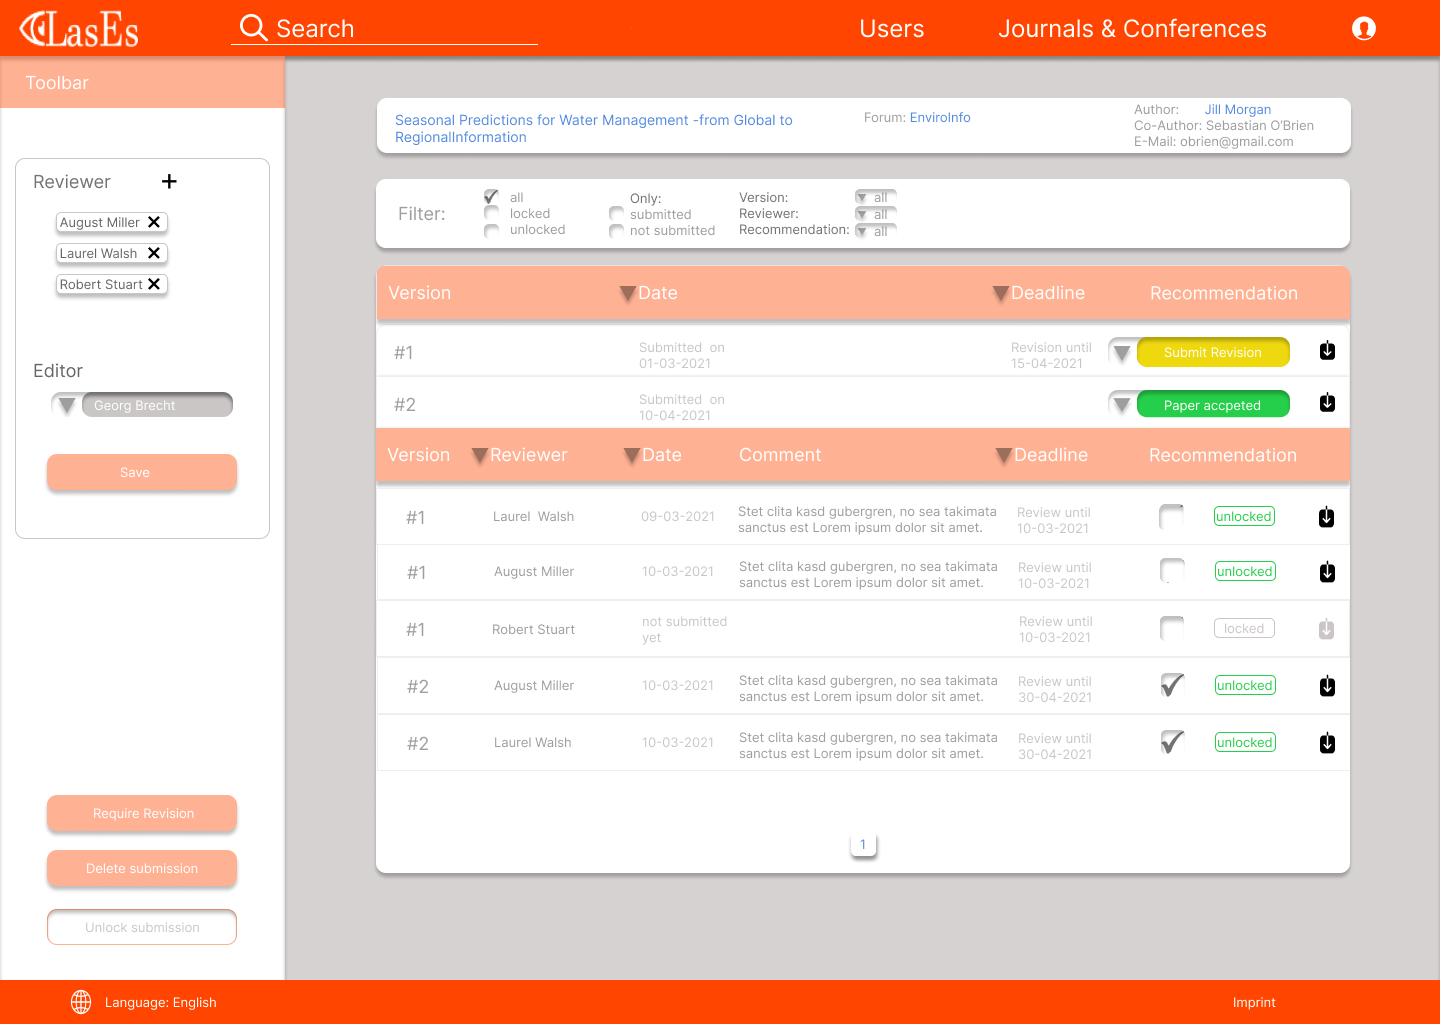
\includegraphics[height=0.75\textheight]{../../docs/Pflichtenheft/graphics/Submission-png}
    \end{frame}


    \section{Libraries}
    \begin{frame}{Basis}
        Es gibt 137,000 python libraries, zu Java habe ich keine Zahlen gefunden aber sind vermutlich noch viel mehr.
        Diese würden uns vermutlich viele QOL Features anbieten.
        Damit man für das Hosten Anwendung kein eigenes Rechenzentrum anmieten muss, haben wir uns für ein paar wenige entschieden.
        Wir garantieren Ihnen: Unsere Anwendung wird ein Leichtgewicht.
        Was nicht bedeutet, dass es nicht mit Schwergewichtsboxern mithalten kann.
        \begin{itemize}
            \item Mojarra v3.0.1
            \item JBoss Weld v4.0.2
            \item PostGreSQL JDBC v42.3.1
            \item Jakarta Mail API v2.0.1
        \end{itemize}
    \end{frame}

    \begin{frame}{Quality of Life}
        \begin{itemize}
            \item Primefaces v10.0.0
            \item Bootstrap v5.1.3
        \end{itemize}
    \end{frame}

    \begin{frame}{Testing}
        \begin{itemize}
            \item JUnit v5.8.1
            \item Mockito v4.0.0
            \item Selenium v4.0.0
        \end{itemize}
    \end{frame}


    \section{Navigationsstruktur}
    \begin{frame}{Navigationsgraph}
        \centering
        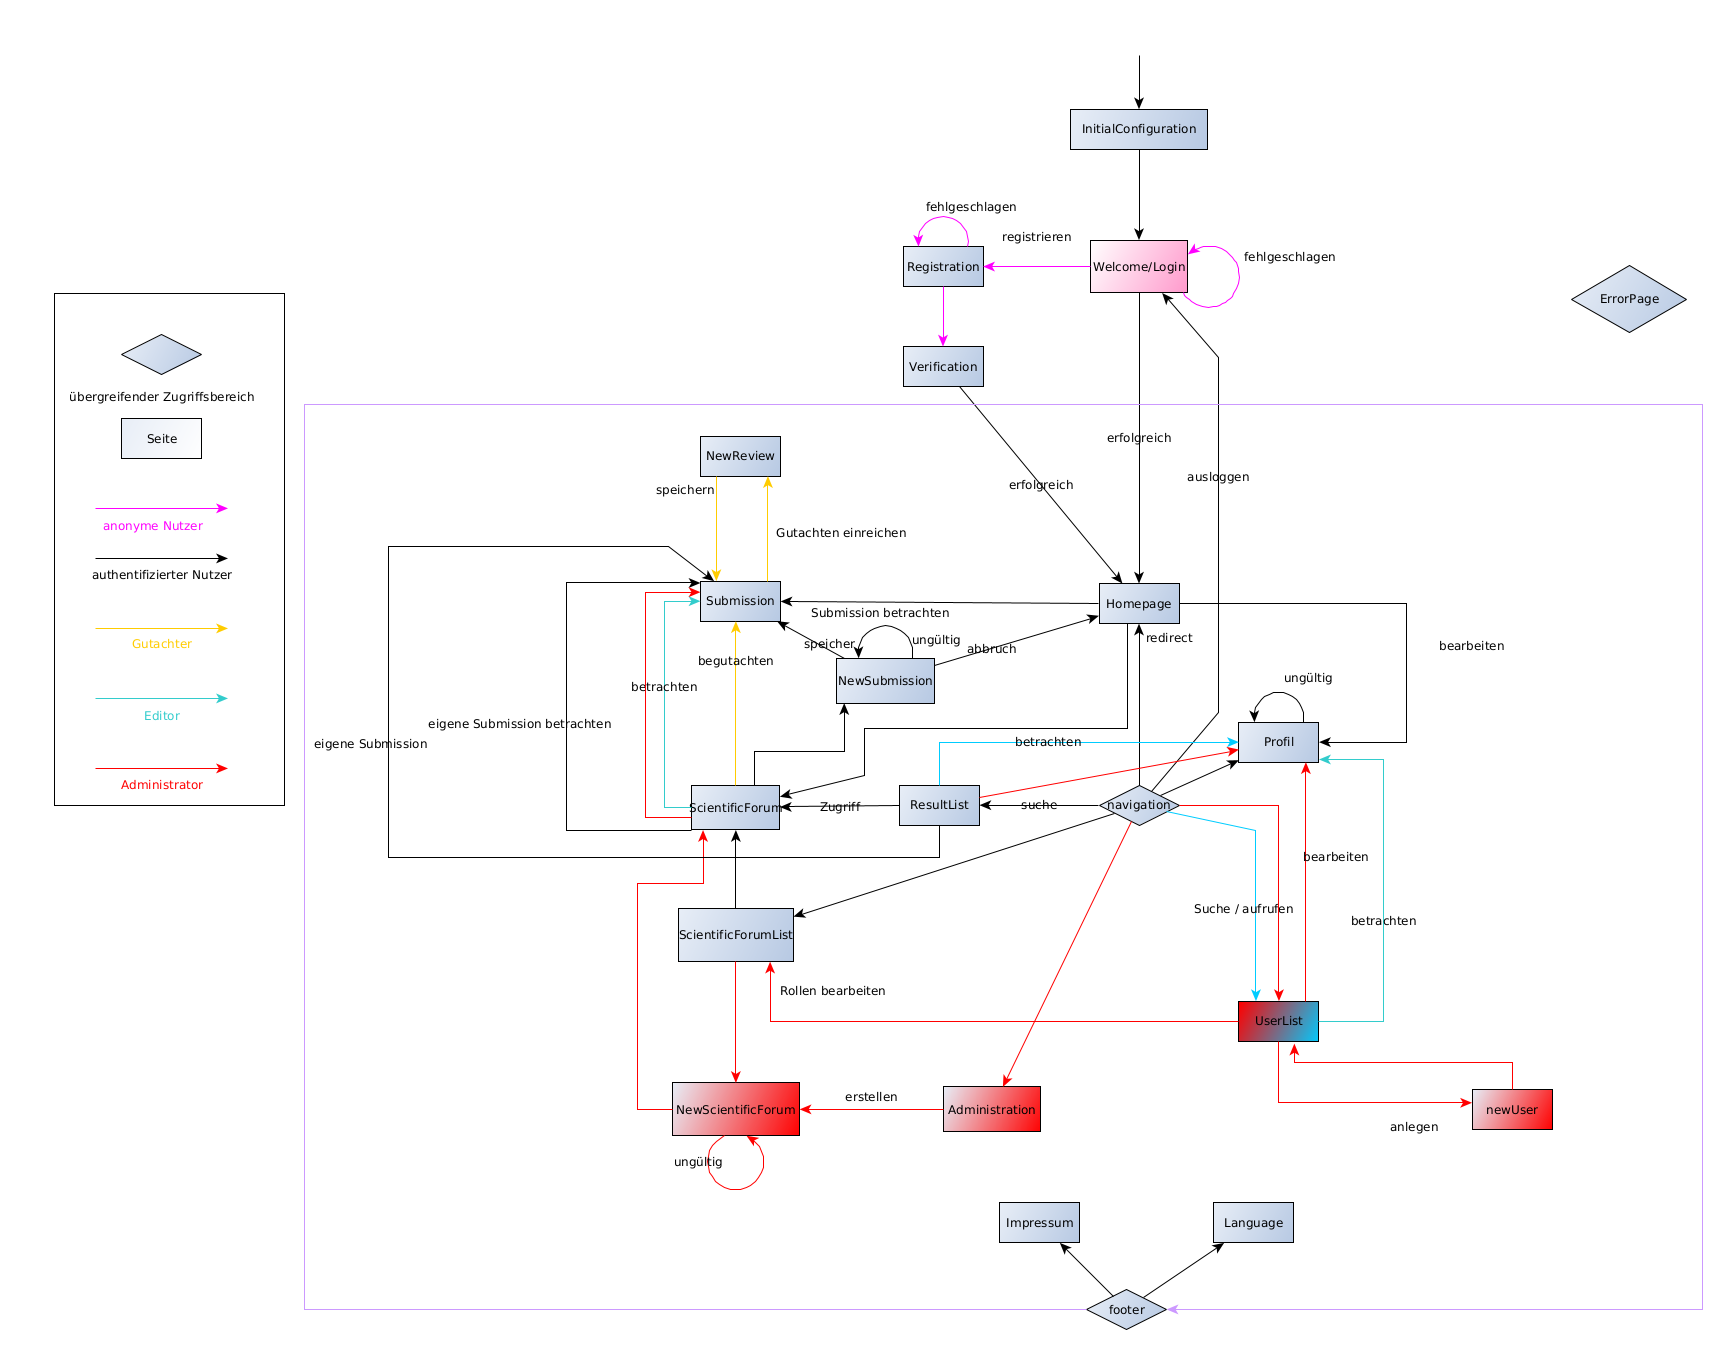
\includegraphics[height=0.8\textheight]{../../docs/Pflichtenheft/graphics/benutzerFlussyEd-png}
    \end{frame}


    \section{Erweiterbarkeit}

    \begin{frame}{Erweiterbarkeit}
        \pause
        \begin{itemize}
            \item Anforderung von Revisionen
            \pause
            \item Mehrsprachige Anwendung
        \end{itemize}
    \end{frame}

    \begin{frame}{Abgrenzungskriterien}
        \pause
        \begin{itemize}
            \item Eigene Anwendung zur Betrachtung der Paper
            \pause
            \item Keine Publikationssoftware oder Lizenzierung
        \end{itemize}
    \end{frame}


    \section{Testing}
    \begin{frame}{Testabläufe}
        \pause
        Setup:
        \begin{itemize}
            \item mehrere Nutzer
            \item Testmodus (für E-Mailbestätigungen)
        \end{itemize}

        \pause

        Ablauf:
        \begin{itemize}
            \item Anlegen einer Konferenz \textbf{(Administrator)}
            \item Einreichung von Paper mit Ko-Autor \textbf{(Nutzer)}
            \item Editor kümmert sich um Gutachteraquirierung \textbf{(Editor \& Gutachter)}
        \end{itemize}
    \end{frame}

    \begin{frame}{Diskussion}
        \centering
        
\includegraphics[width=0.7\linewidth]{../../docs/Pflichtenheft/graphics/LasEs-logo}
    \end{frame}

\end{document}
